% ACIIDS 2027 (Springer LNAI) -- full paper. Limit: 12-15 pages including figures, tables and
% references, Springer LNCS/LNAI template, PDF via EasyChair, deadline 31 Oct 2026 (extended).
% The call does not ask for anonymisation; author names are placeholders to fill in.
\documentclass[runningheads]{llncs}

\usepackage{amsmath,amssymb,amsfonts}
\usepackage{graphicx}
\usepackage{booktabs}
\usepackage{array}
\newcolumntype{L}[1]{>{\raggedright\arraybackslash}p{#1}}
\usepackage{multirow}
\usepackage{algorithm}
\usepackage{algpseudocode}
\usepackage{url}
\usepackage[hidelinks]{hyperref}
\usepackage{cite}
\usepackage{caption}
\captionsetup{font=small}

\graphicspath{{figures/}}
\renewcommand{\topfraction}{0.9}
\renewcommand{\textfraction}{0.07}
\renewcommand{\floatpagefraction}{0.8}
\setcounter{topnumber}{3}
\setcounter{totalnumber}{5}
\newcommand{\awr}{\textsc{ActiveWR}}
\newcommand{\pp}{\,pp}
\newcommand{\ci}[2]{[#1,\,#2]}

\begin{document}

\title{Winning Is Not Killing: Active Win Rate and Expert Iteration with a Network-Free Kill-Search in Bomberman}

\titlerunning{Winning Is Not Killing: Active Win Rate in Bomberman}
\author{First Author\inst{1} \and Second Author\inst{1} \and Third Author\inst{1}}
\authorrunning{F. Author et al.}
\institute{Affiliation, City, Country\\\email{first.author@example.edu}}

\maketitle

\begin{abstract}
Bomberman agents are usually ranked by win rate, although a game can be won because the opponent destroys itself or is caught by a shrinking arena. We define the active win rate, the share of games won with at least one kill credited to the agent's own bomb, and use it to study how a hand-written kill-search without a neural network can be turned into a fast neural policy. Against a fixed rule-based bot, policy-gradient training with a safety mask reaches 40 to 51 percent active win rate, and over a dozen standard refinements fail a preset gate. A search that looks up to three moves ahead lifts the same network to 94 percent. As a sparse loss inside reinforcement learning the search does not help; dense distillation of its labels does. Three rounds of expert iteration produce a convolutional policy at 92 percent, within one point of its search teacher, with one network evaluation per move. Interventions that raise the win rate by up to 16 points leave the active win rate unchanged. Against frozen neural opponents most games are drawn, and with the correct opponent model a search finds a kill plan in only 16 percent of them.
\end{abstract}

\keywords{Bomberman \and evaluation metrics \and expert iteration \and policy distillation \and reinforcement learning}

% =====================================================================================
\section{Introduction}

Deep reinforcement learning (RL) reaches human or grandmaster level in Atari and StarCraft~II~\cite{mnih2015dqn,vinyals2019alphastar}, but with compute far beyond a single consumer machine. Bomberman, and its research variant Pommerman~\cite{resnick2018pommerman}, is a hard test for model-free RL at small scale: a bomb placed at random kills its owner about 40\% of the time~\cite{gao2019hard}, the reward for a kill arrives many steps after the decision that made it, and decisive moments are rare. Large RL efforts needed hundreds of CPUs~\cite{peng2018continual} or long population-based training~\cite{huynh2024} and still lost to search-based agents~\cite{osogami2019,huynh2024}.

A second problem is \emph{how agents are scored}. Several groups noticed that an agent can collect wins when the opponent kills itself~\cite{gao2019skynet,kartal2018demonstrator,huynh2024,weil2023}, but results are still reported as win rate (WR). An early checkpoint of ours won 52.5\% of 40 four-player games while killing nobody with its own bombs.

This paper reports a controlled study, run on consumer hardware, of how to get a fast neural Bomberman agent that wins by killing. The contributions are:
\begin{itemize}
\item \textbf{C1, a metric.} \awr{}, the probability of winning \emph{and} killing at least one opponent with one's own bomb. WR overstates three of our interventions by 3.75--16\pp{}.
\item \textbf{C2, three uses of one search.} Sparse search labels as an auxiliary RL loss, search at play time and dense distillation of search labels: only the last two help ($-2.75$, $+16.5$, $+16.25$\pp{}), testing two directions proposed by Kartal et al.~\cite{kartal2018demonstrator}.
\item \textbf{C3, expert iteration with a network-free expert.} Three rounds of ``student plus deeper search $\rightarrow$ distil'' raise a plain CNN from 48.25\% to 92.25\% \awr{}; the student--teacher gap shrinks from $-3.75$ to $-0.75$\pp{}.
\item \textbf{C4, controlled negative results} for GAE, PPO clipping, advantage normalisation, reward changes, sudden-death training, group-relative advantages and KL-anchored RL after distillation.
\item \textbf{C5, a draw analysis.} With the correct opponent model, a search finds a kill plan in only 15.9\% of the draws between strong agents.
\end{itemize}
Each building block is known; the contribution is the metric, the controlled comparison under a fixed protocol, and the analysis of where the remaining draws come from. Fig.~\ref{fig:pipeline} summarises the path to the final agent.

\begin{figure}[t]
\centering
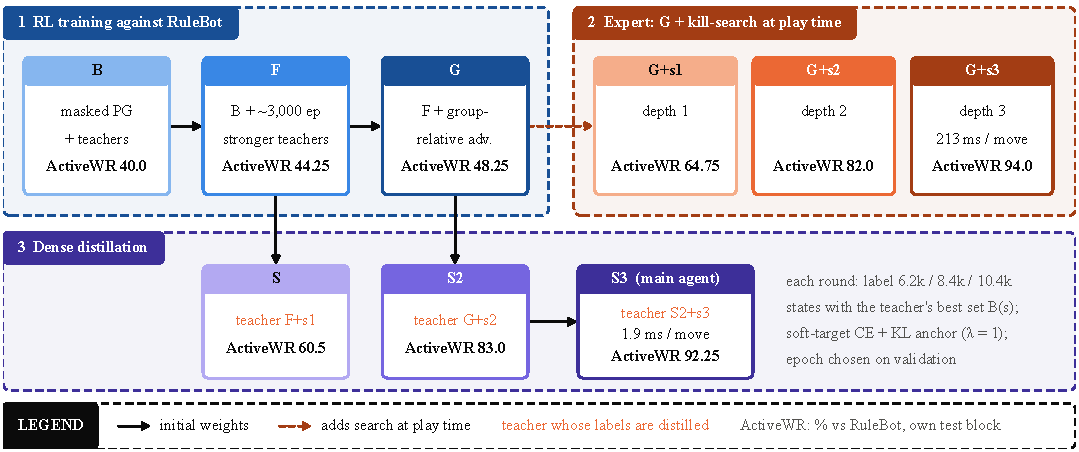
\includegraphics[width=\textwidth]{fig_pipeline.pdf}
\caption{Path from the first RL checkpoint to the final agent. Panel 1: RL-trained CNNs. Panel 2: G with kill-search at play time (the expert); the dashed arrow adds search without changing weights. Panel 3: distilled CNN students; black arrows give the initial weights, the orange label names the teacher whose labels are distilled. Numbers are \awr{} (\%) against RuleBot, each on the model's own single-use test block (Table~\ref{tab:main}).}
\label{fig:pipeline}
\end{figure}

% =====================================================================================
\section{Related Work}

\textbf{RL in Bomberman and Pommerman.} Without action filtering PPO learned nothing in five days; with a filter it learned~\cite{gao2019hard}. Skynet combined PPO, an action filter and reward shaping, and observed that wins often came from opponents killing themselves~\cite{gao2019skynet}. Imitation then RL forgot catastrophically~\cite{meisheri2019}; curriculum and population-based self-play still lost 70--95\% of games to search agents after 200 million steps~\cite{huynh2024}. Backplay~\cite{resnick2018backplay} and continual match training on 220 CPUs~\cite{peng2018continual} attacked the sparse reward.

\textbf{Search in Pommerman.} The NeurIPS 2018 winner used depth-limited tree search with pessimistic opponent scenarios~\cite{osogami2019}. Statistical forward planning produced 59--84\% draws between strong planners~\cite{perezliebana2019}; MCTS with learned opponent models can turn defensive~\cite{weil2023}.

\textbf{Search as a teacher.} UCT decisions trained real-time Atari CNNs~\cite{guo2014uct}. Expert iteration (ExIt)~\cite{anthony2017exit} and AlphaZero~\cite{silver2017agz,silver2017alphazero} alternate a search expert and a network apprentice, with the network guiding the search. In Pommerman, MCTS was a demonstrator inside A3C on an $8\times8$ board~\cite{kartal2018demonstrator,kartal2019safer}. Distillation~\cite{hinton2015distill,rusu2016distill}, DAgger~\cite{ross2011dagger} and kickstarting~\cite{schmitt2018kickstart} give the supervised side of our method.

\textbf{Safety and evaluation.} Masking invalid actions in the logits keeps a valid policy gradient~\cite{huang2022masking}; only potential-based shaping preserves optimal policies~\cite{ng1999shaping}. RL results need confidence intervals over independent units~\cite{henderson2018matters,agarwal2021precipice}; we use the bootstrap~\cite{efron1979bootstrap} over paired boards.

% =====================================================================================
\section{Problem Setting}
\label{sec:setting}

\textbf{Game.} A NumPy re-implementation of Pommerman-style Bomberman on a $9\times9$ board with a border, rigid pillars on (even, even) cells and 70\% wooden walls elsewhere except $3\times3$ spawn zones. Two agents start in opposite corners; actions are STOP, four moves and BOMB. A bomb explodes after 8 steps into a cross of range 2, destroys wooden walls (a power-up appears with probability 0.3), kills agents in the blast and chains into other bombs. A game ends when at most one agent is alive or after 500 steps (draw). Our default sudden-death schedule E closes the arena from the border inwards from step 475 every 25 steps, with a 40-step warning.

\textbf{Observation.} Each agent sees 13 $9\times9$ planes: walls, bomb timers, flames, two power-up types, both positions, free bomb slots, capacity, range, the inverse time until each cell is hit by a forecast blast including chains, and the ring warning.

\textbf{Safety mask and opponent.} Every agent acts through the same safe-action mask $m(s)\in\{0,1\}^6$, which removes moves into cells a forecast blast reaches before the agent can leave and bombs without an escape route. The opponent is a rule-based bot (RuleBot) that dodges, collects items, attacks with the correct blast range and uses the same mask; when no rule applies it picks a random safe move, so its play is stochastic. RuleBot is fixed throughout.

\textbf{Metric.} Let $W$ be the event that the learner is the last agent alive and $K$ that at least one opponent died in a blast credited to a learner bomb (credit follows the owner of the bomb that started a chain). We report $\awr{}(\pi)=\Pr_{\pi}[W\wedge K]$ and decompose every evaluation into active, passive (opponent self-kill) and ring wins, draws, self-kills and other losses. WR $=\Pr[W]$ is secondary.

% =====================================================================================
\section{Method}

All agents share one actor--critic CNN: three $3\times3$ convolutions (32, 64, 64 channels, padding 1), a 256-unit layer, a 6-way actor head and a critic head (1.39M parameters). Logits of unsafe actions are set to $-10^9$ before the softmax, which keeps the policy gradient valid~\cite{huang2022masking}. Actions are \emph{sampled}: argmax play lowered F's \awr{} by 9.25\pp{} \ci{-16.0}{-2.5} and raised draws by 7.5\pp{} on validation.

\subsection{Stage 1: masked policy gradient with auxiliary teachers}
The RL stage trains against RuleBot with Monte-Carlo returns ($\gamma=0.99$) and a learned baseline (REINFORCE with baseline~\cite{williams1992reinforce}; GAE~\cite{schulman2016gae} and PPO clipping~\cite{schulman2017ppo} were tested as variants), an entropy bonus and cross-entropy terms towards four rule-based teachers (escape, combat, navigation, ring safety; weights 0.5, 0.9, 0.4, 0.6). Rewards are event-based ($+4$ per credited kill, $-1$ on death, $-1.5$ extra for a self-kill, small item and wall bonuses); the $+10$ for being last alive is kept only for active wins. A game of about 230 steps has only about 2.2 steps where the actions' search scores differ and 1.25 where some action kills, so we also tried a GRPO-like update~\cite{shao2024grpo} at such \emph{decisive} states: the policy is replayed $K=16$ times for 20 ticks, with outcome $o_k\in\{+1,-1,0\}$ (credited kill, death, neither) and advantage $o_k-\bar o$. The resulting checkpoint G is our best RL policy.

\subsection{Stage 2: network-free kill-search}
For each legal first action, a copy of the game is simulated for 12 ticks (fuse 8 + flame 2 + slack) with the opponent playing RuleBot and the learner only dodging afterwards (Algorithm~\ref{alg:search}). A rollout scores $+1$ if an opponent dies from a learner bomb while the learner lives, $-1$ if the learner dies, else 0. Depth 2 or 3 adds learner moves before dodging and is expanded only when no shorter plan kills. The search is skipped unless an opponent is within Manhattan distance 6, and the CNN's sampled action is kept unless another action scores strictly higher.

\begin{algorithm}[t]
\caption{Kill-search of depth $d$ (play time)}
\label{alg:search}
\small
\begin{algorithmic}[1]
\Require state $s$, mask $m$, CNN action $a_0$, depth $d$, horizon $H=12$
\If{no opponent within distance 6} \Return $a_0$ \EndIf
\For{$a$ with $m_a(s)=1$}
  \State $v_1(a)\gets$ \Call{Rollout}{$s,[a],H$} \Comment{RuleBot opponent}
\EndFor
\If{$\max_a v_1(a)>v_1(a_0)$} \Return $\arg\max_a v_1(a)$ \EndIf
\For{$\ell=2,\dots,d$} \Comment{only if no shorter kill}
  \For{safe prefixes $(a,b_2,\dots,b_\ell)$}
    \State $v_\ell(a)\gets\max$ \Call{Rollout}{$s,(a,b_2,\dots,b_\ell),H$}
  \EndFor
  \If{some $v_\ell(a)>0$ and $v_\ell(a_0)\le 0$} \Return first move of a kill plan \EndIf
\EndFor
\State \Return $a_0$
\end{algorithmic}
\end{algorithm}

\subsection{Stage 3: dense distillation and expert iteration}
The teacher (current student + depth-$d$ search) plays 3{,}000 games against RuleBot on fresh boards. At every learner step the search scores all legal actions; a \emph{decision state} is one where the scores differ, and its target spreads mass uniformly over the best set $B(s)=\arg\max_{a:m_a(s)=1}v(a)$. With probability 0.05 an ordinary state is stored as an \emph{anchor} with the starting network's logits. The student starts from the previous network and minimises
\begin{equation}
\mathcal{L}=\mathbb{E}_{\mathcal{D}_{\mathrm{dec}}}\!\Bigl[-\textstyle\sum_a q(a\mid s)\log\pi_\theta(a\mid s)\Bigr]+\lambda\,\mathbb{E}_{\mathcal{D}_{\mathrm{anc}}}\mathrm{KL}\bigl(\pi_{\mathrm{ref}}\Vert\pi_\theta\bigr)
\end{equation}
with $\lambda=1$, Adam ($10^{-4}$), batch 256 and 8 or 16 epochs; the epoch is chosen on validation. Round 1 distils F + depth 1 into S, round 2 G + depth 2 into S2, round 3 S2 + depth 3 into S3 (6{,}171, 8{,}449 and 10{,}425 decision states). Unlike ExIt~\cite{anthony2017exit}, the expert never uses the network's prior or value; the student improves only because the expert also plays the student's own moves where the search is indifferent, keeping the data close to the student's state distribution~\cite{ross2011dagger}.

% =====================================================================================
\section{Evaluation Protocol}
\label{sec:protocol}

Every experiment follows the same pre-specified protocol (fixed in our repository before each run, not in a public registry). (i) Configuration, source hashes and selection rule are written before training. (ii) Checkpoints are selected only on validation seed 21000. (iii) Selected models are tested \emph{once} on a fresh block of 200 boards, each played from both corners (400 games); a test block is never reused. (iv) Models are compared with a paired bootstrap~\cite{efron1979bootstrap} over boards ($10^4$ resamples). (v) A change is accepted only if $\hat\Delta\ge+5$\pp{}, the lower CI bound is above zero and self-kills rise by at most 1\pp{}. One 400-game block of the same pair varies by about $\pm5$\pp{} across blocks, which is why the gate needs both a margin and a positive bound. RQ1 asks how much WR misjudges agents, RQ2 which use of a search transfers its strength to a CNN, RQ3 how close expert iteration brings a CNN to the search, RQ4 why RL refinements fail, and RQ5 whether draws between strong agents are missed chances.

% =====================================================================================
\section{Results}

\begin{table}[t]
\centering
\caption{Main results against RuleBot ($9\times9$, 1v1, schedule E, 400 test games per model on its own single-use test block; only rows on the same block are compared inferentially). CI: 95\% bootstrap over boards. B: masked PG + teachers; F: B + 3{,}000 RL episodes; G: F + group-relative advantage; G+s$d$: G with kill-search of depth $d$; S, S2, S3: distillation rounds 1--3. $^\ast$B's original test predates sudden death; the row uses a cross-check block.}
\label{tab:main}
\scriptsize
\setlength{\tabcolsep}{4pt}
\begin{tabular}{@{}lrrrrrr@{}}
\toprule
Agent & Block & \awr{} \% [95\% CI] & WR \% & Passive/ring \% & Draw \% & Self-kill \% \\
\midrule
B$^\ast$ & 60000 & 40.0 \ci{35.0}{45.0} & 64.0 & 24.0 & 22.5 & 0.5 \\
F & 43000 & 44.25 \ci{39.25}{49.25} & 63.5 & 19.25 & 25.0 & 1.0 \\
G & 46000 & 48.25 \ci{43.5}{53.25} & 69.0 & 20.75 & 23.25 & 0.75 \\
\midrule
G+s1 & 46000 & 64.75 \ci{60.25}{69.25} & 84.0 & 19.25 & 15.25 & 0.0 \\
G+s2 & 47000 & 82.0 \ci{78.25}{85.75} & 93.75 & 11.75 & 5.75 & 0.0 \\
G+s3 & 49000 & \textbf{94.0} \ci{91.75}{96.25} & 99.5 & 5.5 & 0.25 & 0.0 \\
\midrule
S & 43000 & 60.5 \ci{55.25}{65.75} & 78.5 & 18.0 & 18.0 & 1.0 \\
S2 & 48000 & 83.0 \ci{79.5}{86.5} & 90.25 & 7.25 & 7.0 & 0.25 \\
S3 & 57000 & \textbf{92.25} \ci{89.5}{94.75} & 98.0 & 5.75 & 0.5 & 0.25 \\
\bottomrule
\end{tabular}
\end{table}

\begin{figure}[t]
\centering
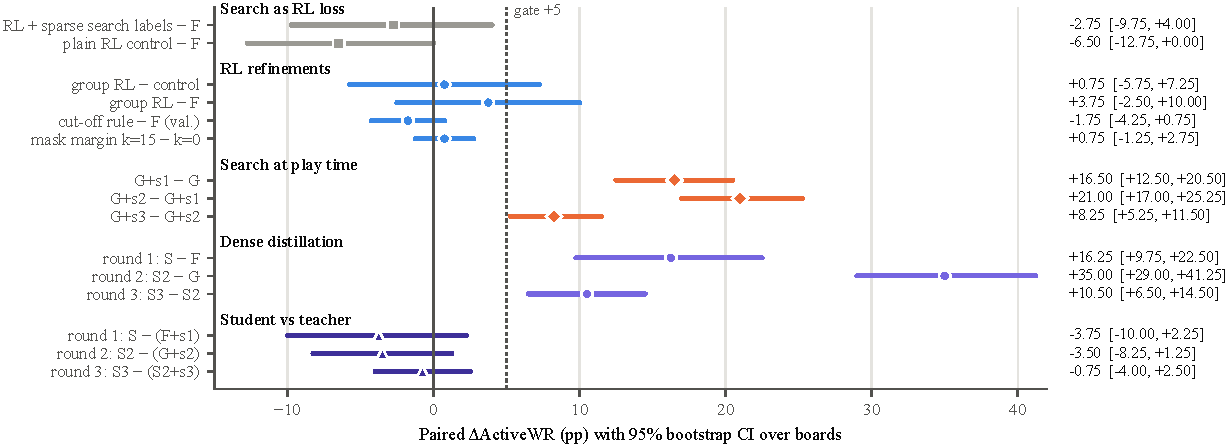
\includegraphics[width=\textwidth]{fig_forest.pdf}
\caption{Paired $\Delta$\awr{} with 95\% bootstrap CIs over boards, recomputed from per-game logs. Dashed line: +5\pp{} gate. ``val.'' marks a validation-block comparison.}
\label{fig:forest}
\end{figure}

\subsection{RQ1: win rate misjudges agents}
\label{sec:rq1}
Fig.~\ref{fig:wr} shows four interventions measured with both metrics on paired boards. A learner-side mask margin of 15 steps for the shrinking ring raised WR by $+10.75$\pp{} \ci{6.25}{15.5} but \awr{} by only $+0.75$ \ci{-1.25}{2.75}: deaths in the ring fell from 116 to 76 of 400, so the gain was survival. A rule that makes the learner stand on the opponent's escape cell raised WR by $+3.75$ while \awr{} fell by 1.75, turning 16 of F's active wins into passive ones. Turning sudden death on adds 16\pp{} of WR to G with no \awr{} change. Fig.~\ref{fig:outcomes} shows the pattern across all milestones.

\begin{figure}[t]
\centering
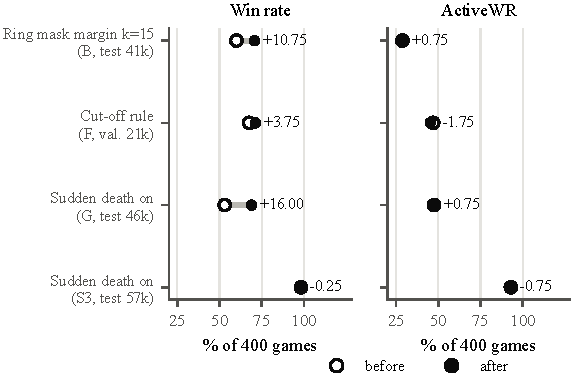
\includegraphics[width=0.85\textwidth]{fig_wr_vs_active.pdf}
\caption{Win rate versus \awr{} for the same paired games; labels give after-minus-before (pp).}
\label{fig:wr}
\end{figure}

\begin{figure}[t]
\centering
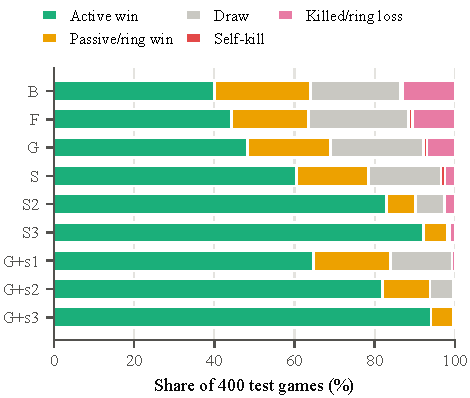
\includegraphics[width=0.85\textwidth]{fig_outcomes.pdf}
\caption{Outcome composition of the 400-game tests of Table~\ref{tab:main}. RL checkpoints win many games passively or by the ring; students and search agents win by killing.}
\label{fig:outcomes}
\end{figure}

\subsection{RQ2: three uses of the same search}
Table~\ref{tab:three} compares three ways to use the depth-1 kill-search. As a sparse auxiliary loss inside RL (labels only where the search disagrees with the CNN, about 0.9 per episode, each used once) it did not help. At play time it adds $+16.5$\pp{}. Densely distilled (about 6{,}200 decision states with counter-examples, 8 epochs), it moves the CNN by $+16.25$\pp{} with no search at play time. The student learned the condition ``only BOMB kills here'': the probability of the best move on held-out decision states rose from 0.52 to 0.91, while $P(\text{BOMB})$ on ordinary states stayed at 0.088 $\rightarrow$ 0.095.

\begin{table}[t]
\centering
\caption{Three uses of the same depth-1 kill-search (paired \awr{} differences, own test blocks).}
\label{tab:three}
\scriptsize
\setlength{\tabcolsep}{3pt}
\begin{tabular}{@{}llrl@{}}
\toprule
Use & Comparison & $\Delta$\awr{} [95\% CI] & Block \\
\midrule
Sparse loss in RL & search arm $-$ F & $-2.75$ \ci{-9.75}{+4.0} & 42000 \\
Search at play time & G+s1 $-$ G & $+16.5$ \ci{+12.5}{+20.5} & 46000 \\
Dense distillation & S $-$ F & $+16.25$ \ci{+9.75}{+22.5} & 43000 \\
\bottomrule
\end{tabular}
\end{table}

\subsection{RQ3: expert iteration with a network-free expert}
\textbf{Search depth.} Fig.~\ref{fig:depth} links depths on shared test blocks: depth 1 adds $+16.5$ over G, depth 2 adds $+21.0$ \ci{17.0}{25.25} over depth 1 and depth 3 adds $+8.25$ \ci{5.25}{11.5} over depth 2, nearly removing draws (5.75 $\rightarrow$ 0.25\%). The gains come from \emph{creating} a kill (step, then bomb): depth-1 search plateaus near 65\% whatever CNN it wraps.

\begin{figure}[t]
\centering
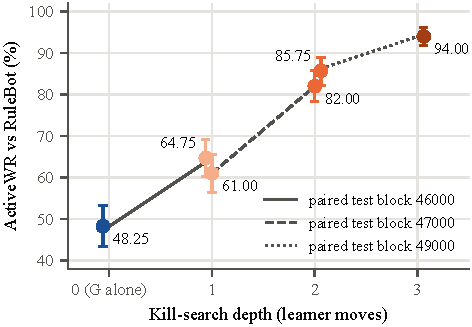
\includegraphics[width=0.85\textwidth]{fig_search_depth.pdf}
\caption{\awr{} versus kill-search depth around G; each line style joins two agents tested on one paired block. Error bars: 95\% CIs over boards.}
\label{fig:depth}
\end{figure}

\textbf{Iterated distillation.} Each round closes most of the student--teacher gap: S $-$ (F+s1) $=-3.75$ \ci{-10.0}{2.25}, S2 $-$ (G+s2) $=-3.5$ \ci{-8.25}{1.25}, S3 $-$ (S2+s3) $=-0.75$ \ci{-4.0}{2.5} (versus G+s3: $-1.75$), while the teachers get stronger. Round gains are $+16.25$, $+35.0$ \ci{29.0}{41.25} and $+10.5$ \ci{6.5}{14.5}. The S3 gain is active: passive wins change by $-1.5$ \ci{-4.5}{1.5}, draws by $-6.25$, games are shorter (131 versus 202 steps) and disabling sudden death gives the same $+10.75$. Repeating round 3 with new collection boards and train seeds gives S3 $-$ S2 of $+10.5$, $+9.0$ and $+9.25$ on a shared fresh test block (s.d.\ 0.8); all three pass the gate. Held-out agreement with the teacher's best set rises from 60.5 to 94.0\% in round 2 and from 74.8 to 89.8\% in round 3, while the KL to the reference policy on anchors stays below 0.11 nats. The main fix is movement, not bombing: G walks the opposite way to the search in up to 67\% of states and almost never stops when STOP is best, while BOMB is already right in 94\%.

 A stronger base does not make the search stronger: S2+s3 versus G+s3 on validation is $-5.0$ \ci{-11}{1}. A depth-3 decision costs 213\,ms on one CPU thread against 1.9\,ms for one S3 forward pass and sample (about $115\times$).

\subsection{RQ4: ablations and controlled negative results}
\label{sec:rq4}
Fig.~\ref{fig:forest} plots the main gated comparisons. From B, 200-episode arms with teacher variants, advantage normalisation, GAE, reward changes and PPO clipping stayed within a few points of B, and training under sudden death lowered \awr{} by 2.25\pp{}. From F, 3{,}000 more RL episodes did not help ($-6.5$), nor did group-relative advantages on decisive states ($+0.75$ against the matched control), although they raised the kill rate at those states by $+7.12$\pp{} \ci{4.86}{9.72}. Pushing BOMB at narrow states raised $P(\text{kill move})$ from 0.72 to 0.97 but not kills per game, and no KL weight separated ``bomb at the right moment'' from ``bomb anywhere''. Self-play RL from the distilled S2 erased the skill (\awr{} 83.75 $\rightarrow$ 65.0 and 57.5), and a global KL anchor kept only 2.5\pp{} of it.

\subsection{RQ5: draws between strong agents}
\label{sec:rq5}
Against frozen CNNs (S2, G, S3) S3 still draws 53--64\% of validation games, mostly at the 500-step limit (Fig.~\ref{fig:cnn}); against RuleBot it draws under 1\% with a median game of 105 steps. To ask whether these draws hide missed kills, we replayed 195 draws of S3 and ran the depth-3 search at every fifth state with two opponent models (Fig.~\ref{fig:draws}). Under the RuleBot model the search sees a kill plan in 90.3\% of draws; with the opponent's own CNN as model, in only 15.9\% \ci{9.9}{22.7}, while all 20 control active wins contain a plan. Starting the ring earlier did not help either: \awr{} changed by $-1.42$ to $-0.17$\pp{}, and 80--87\% of the remaining draws became simultaneous deaths in the last ring. Both agents use the same safety mask, so a CNN almost always keeps an exit and a forced kill rarely exists.

\begin{figure}[t]
\centering
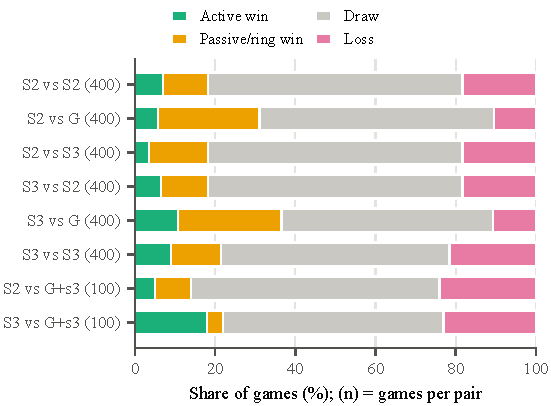
\includegraphics[width=0.85\textwidth]{fig_cnn_matchups.pdf}
\caption{Outcomes of CNN-versus-CNN and CNN-versus-search games on validation boards (learner first; games per pair in brackets).}
\label{fig:cnn}
\end{figure}

\begin{figure}[t]
\centering
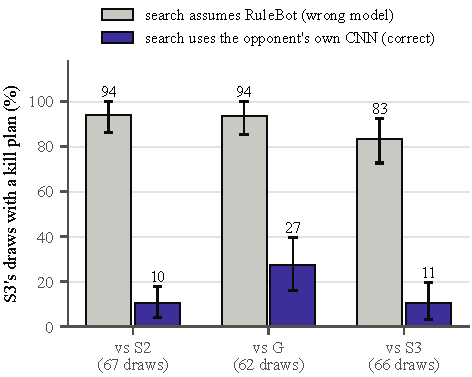
\includegraphics[width=0.85\textwidth]{fig_draw_probe.pdf}
\caption{Share of S3's draws against each CNN in which the depth-3 search finds a kill plan, under the wrong (RuleBot) and the correct (opponent's own CNN) opponent model. Error bars: 95\% bootstrap CIs over games.}
\label{fig:draws}
\end{figure}

\subsection{Larger board and free-for-all}
\label{sec:ffa}
Interpolating S3 to $11\times11$ gives 46.25\% \awr{}; one distillation round on 200 teacher games produced S3-11 with 87.25\% on a fresh test block, $+41.0$ \ci{34.5}{47.25}, but against frozen CNNs only $+3.83$ \ci{1.92}{5.83}. In free-for-all against RuleBots on a fresh block (seed 59000; 180 and 160 games), S3 reached 82.8 \ci{76.1}{88.9} \awr{} with three agents on $9\times9$, $+46.7$ \ci{36.1}{56.7} over G on the same boards, although it was distilled from 1v1 games only; with four agents on $11\times11$, S3-11 reached 59.4 \ci{50.6}{68.1} ($+41.9$ over G). Against fair shares of 33\% and 25\%, 94\% and 93\% of the students' wins are active, against 64\% and 58\% for G: opponents also die by their own bombs, by each other or in the ring, so WR flatters weak agents most. G+s3 reached 94.4 and 86.3 on an earlier block, so the gap to the search grows outside 1v1.

% =====================================================================================
\section{Discussion}

\textbf{Why dense distillation works where RL does not.} Decisive states are rare, and Monte-Carlo policy gradient spreads credit over all steps~\cite{williams1992reinforce}. A sparse label used once is too little signal; the same labels stored and replayed for several epochs, with counter-examples where BOMB is wrong, teach a conditional rule that RL's one-sided signal could not separate. This matches the finding that more demonstrations matter more than better ones~\cite{kartal2019safer}. RL after distillation forgets because our anchors used fixed weights and the KL on decision states was about ten times larger than on ordinary ones; kickstarting needed a decaying weight~\cite{schmitt2018kickstart}, and imitation-then-PPO in Pommerman also forgot~\cite{meisheri2019}.

\textbf{The ceiling and generality.} The search never uses the network, so expert iteration lacks ExIt's step where the apprentice improves the expert~\cite{anthony2017exit}; S3 approaches but does not pass 94\%. All agents were tested in one environment against one scripted opponent that the search models. The skill survives free-for-all and, after one more distillation round, a larger board, but not frozen CNN opponents. The study therefore supports a claim about turning a search that models a known opponent into a fast network, not about strength against arbitrary opponents.

\begin{table}[t]
\centering
\caption{Reported results of published Pommerman agents and of ours. Settings differ (Pommerman: $11\times11$, 10-step bombs, kicking, 800-step games, partial observation in team mode; ours: no kicking, 8-step bombs, 500 steps with sudden death, full observation), so rows position results and are not a head-to-head comparison. No published work reports \awr{}.}
\label{tab:sota}
\footnotesize
\setlength{\tabcolsep}{3pt}
\scriptsize
\begin{tabular}{@{}L{0.15\textwidth}L{0.18\textwidth}L{0.15\textwidth}L{0.22\textwidth}L{0.24\textwidth}@{}}
\toprule
Work & Setting & Opponents & Method & Reported result \\
\midrule
Gao 2019~\cite{gao2019hard} & FFA / team & 3 SimpleAgents / team & PPO + action pruning & WR 40--43\% (FFA), 65--76\% (team) \\
Perez-Liebana 2019~\cite{perezliebana2019} & FFA, full observation & 3 rule-based agents & MCTS / RHEA & WR 46.5\% / 33.0\% \\
Weil 2023~\cite{weil2023} & official FFA & 3 SimpleAgents & MCTS + learned model & WR 61--78\%, ties 12--34\% \\
Meisheri 2019~\cite{meisheri2019} & team $2\times2$, partial & SimpleAgent team & imitation $\rightarrow$ PPO & WR 77.8\% \\
Osogami 2019~\cite{osogami2019} & team $2\times2$ & SimpleAgent team & depth-1 search, pessimistic & WR 92.6--99.7\% \\
Huynh 2024~\cite{huynh2024} & team $2\times2$, partial & SimpleAgent; search agent & PPO + LSTM, PBT, 200M steps & WR 98.85\%; 30.0\% vs search \\
\midrule
Ours, G+s3 & FFA $11\times11$, 4 agents & 3 RuleBots & G + network-free kill-search & WR 88.8\%, \awr{} 86.3\% \\
Ours, S3-11 & FFA $11\times11$, 4 agents & 3 RuleBots & distilled CNN, no search & WR 63.8\%, \awr{} 59.4\% \\
Ours, S3 & 1v1 $9\times9$ & RuleBot & distilled CNN, no search & WR 98.0\%, \awr{} 92.25\% \\
\bottomrule
\end{tabular}
\end{table}

\textbf{Comparison with published agents.} No agent was run in both environments, so Table~\ref{tab:sota} positions results rather than ranking them. Pommerman is the broader benchmark, but three differences make our numbers conservative. \emph{The criterion is stricter}: published results count all wins; under that criterion S3 would report 98.0\% instead of 92.25\%. \emph{Waiting is not rewarded}: bombs explode after 8 steps instead of 10 and a ring closes the arena, whereas in Pommerman most ties come from the 800-step limit~\cite{weil2023}. \emph{The budget is small}: S3 needs one forward pass per move, while the strongest learning agent in Pommerman needed 200 million steps and still wins only 30\% against a depth-1 search~\cite{huynh2024,osogami2019}. Within these caveats the ordering matches the literature: search leads learning, and in four-agent free-for-all the network-only S3-11 (63.8\%) lies within the range of MCTS with learned models (61--78\%)~\cite{weil2023}. RuleBot and SimpleAgent are both weak heuristics below the fair share (11.9\% and about 20\%~\cite{resnick2018pommerman}) but were never played against each other.

% =====================================================================================
\section{Limitations}
(1) Only distillation round 3 was replicated over training seeds (three seeds, all pass); other arms used one seed, so their intervals measure variation over boards, not training runs~\cite{henderson2018matters,agarwal2021precipice}. (2) The reference opponent is RuleBot, and the search assumes RuleBot. (3) Milestones in Table~\ref{tab:main} come from different test blocks. (4) Policies are sampled, so numbers reproduce bit-for-bit only with the same torch version. (5) Free-for-all and $11\times11$ results are single runs. (6) The agents were not run in the official Pommerman environment or against SimpleAgent.

\section{Conclusion}
In Bomberman, win rate rewards survival and opponent mistakes; \awr{} measures an agent that wins by killing. Measured this way, model-free RL with a safety mask stalls below about 50\%, a short network-free kill-search reaches 94\%, and distilling its labels three times gives a single CNN at 92.25\% that needs one forward pass per move. Against equally careful neural opponents most games remain draws, mainly because of the game's rules.

\subsubsection*{Statements.}
\noindent\textbf{Data and code.} Code, run registrations, per-game logs and figure scripts: anonymised repository \url{https://anonymous.4open.science/r/ANONYMOUS-ID}. Supplementary material gives the observation planes, the game-length distributions and the RL training curves.
\noindent\textbf{Use of AI tools.} An AI assistant helped draft and edit the text and write plotting code; the authors designed and ran the experiments, checked every number against the logs and take responsibility for the content.

\bibliographystyle{splncs04}
\bibliography{references}

\end{document}
